The goal of JL is to presere $\ell_{2}$ distances. However, depending
on what property you care about, there will be different linear
dimensionality reduction techniques appropriate for your task. \\ 

\noindent Common linear dimensionality reduction techniques:
\begin{itemize}
\item RP (Random Projection)
\item PCA (Principal Component Analysis)
\item LDA (Linear Discriminate Analysis)
\item MDS (Multi-dimensional Scaling)
\item ICA/BSS (Independent Component Analysis/Blind Source Separation)
\item CCA (Canonical Correlation Analysis)
\item DML (Distance Metric Learning)
\item Factor (Factor Analysis)
\item NMF/MF ((Non-negative) Matrix Factorization)
\item Feature Selection
\end{itemize}

\section{RP (Random Projection)}
\subsubsection*{Method}
For random projection, $P\in \mathbb{R}^{d\times D}$ with $P_{ij} =
\mathcal{N}(0,1)$. i.e. 
\[
P = 
\begin{bmatrix}
    \mathcal{N}(0,1) & \mathcal{N}(0,1) & \dotsm\ \\
    \vdots & \ddots & \\
\end{bmatrix}
\]
If a projection matrix is wanted, apply Gram-Schmidt to $P$.

\subsection{Practical application}
PCA has time complexity $O(n^3)$, if we assume both the number of data
points and the number of features are equal to $n$. In practice, if we
are working with large amounts of data our first instinct to speed up
PCA might be to subsample the data, i.e. if our dataset has 10k
samples in $\mathbb{R}^{10k}$, randomly subsample 1k points and
perform PCA on this reduced dataset. However, the quality of the
$k^{\rm th}$ eigenvector of the subsampled data decays with respect to
the $k^{\rm th}$ eigenvector of the full dataset. While the first
eigenvector of the subsampled and full dataset will be similar, all
subsequent eigenvectors of the subsampled data will be of worsening
quality.  

The better approach to speeding up PCA is to first do a random
projection, and then perform PCA. While the distances between points
will be distorted within 1 $\pm$ $\epsilon$, the quality of the
eigenvectors will be better.

Random Projection plays a major role in processing images from
single-pixel cameras. These cameras use a method called compressive
sampling, which looks to reconstruct the optical signal. 
Specifically, random projection helps with a technique called 
smashed filters (as opposed to matched filters), which benefits from
the fact that random sampling preserves the original structure of the
data with high probability since it maintains inter-point distances. 
To learn more about this process, see "Single-Pixel Imaging via 
Compressive Sampling" \cite{duarte}.

\section{PCA~(Principal Component Analysis)}
\subsection{Outline}
Input Data: $x_1,x_2,...,x_n \in \mathbb{R}^d$\\

\noindent Goal: Find the best linear transformation $\phi:
\mathbb{R}^d \rightarrow \mathbb{R}^k$ that best maintains
reconstruction accuracy. Equivalently, minimize aggregate residual
error.\\ 

\noindent Define: $\Pi^k: \mathbb{R}^d \rightarrow \mathbb{R}^d$ to
minimize $\frac{1}{n} \sum_{i=1}^n ||x_i - \Pi^k (x_i)||^2$\\

\begin{figure}[h!]
\begin{center}
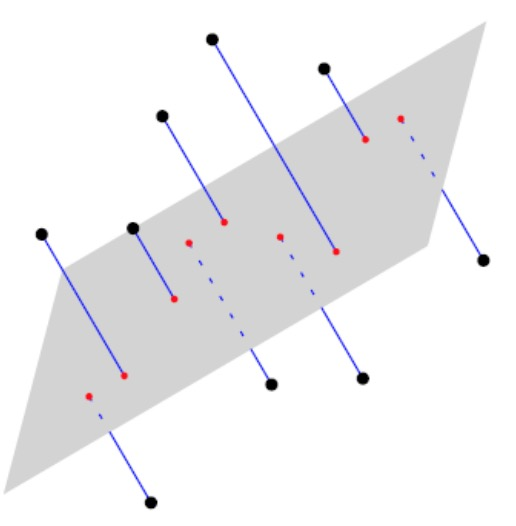
\includegraphics[width=0.5\textwidth]{chapter_6/files/projections.jpg}
\caption{An illustration of PCA}
\end{center}
\end{figure}
\subsection{Method}
A $k$ dimensional subspace can be represented by $q_1,...,q_k \in
\mathbb{R}^d$ orthonormal vectors. 
The projection of any $x\in \mathbb{R}^d$ into $span\{q_1,...,q_k\}$
is given by 
\[
\underbrace{(\sum_{i=1}^k q_i q_i^T)}_{\Pi^k}x = \sum_{i=1}^k
(q_i\cdot x)q_i 
\]
To represent it in $\mathbb{R}^k$ (corresponding to basis $\{q_1,...,q_k\}$), the
coefficients are: $(q_1,x),...,(q_k,x)$.

\subsubsection{The $k$ = 1 case}
In $k=1$ case, the objective is the following:\\

$$\underset{||q||=1}{\min} \frac{1}{n} \sum_{i=1}^n
||x_i - (qq^T)x_i||^2$$

\noindent Equivalently,\\

$$\underset{||q||=1}{\max}q^T(\frac{1}{n} XX^T)q$$

\noindent where $\frac{1}{n}XX^T$ is the covariance of data, if the
data is mean-centered. The solution is the top eigenvector
$(1/n)XX^T$.\\ 

\noindent \textbf{Remark}: For any $q$, the quadratic form
$q^T(\frac{1}{n}XX^T)q$ is the empirical variance of data in the
direction $q$. 

\subsubsection{General $k$ case}
The optimization problem is the following
\begin{align*}
\min & \quad tr(XQQ^TX^T)\\
s.t. & \quad Q^TQ = I\\
 &  \quad rank(Q) = k
\end{align*}
And the solution is basically the top $k$ eigenvectors of the matrix $XX^T$. 

\section{LDA~(Linear Discriminate Analysis)}
\subsection{Motivation}
\subsubsection{Input Data}
Suppose our data $X$ have two labels $+$ and $-$, the group of data labeled $+$ is defined as $C_{+}$ and similarly define $C_{-}$.

\subsubsection{Goal}
The goal of \textbf{LDA} is to project the means of the two groups onto a $1$-dimensional subspace that separating their distance as much as possible.


\subsection{Method}
 Define the group means of $C_{+}$ and $c_{-}$:
\begin{center}
	$\mu_{+} = \frac{1}{|C_{+}|}\sum\limits_{x \in C_{+}}x$\\
	$\mu_{-} = \frac{1}{|C_{-}|}\sum\limits_{x \in C_{-}}x$
\end{center}
Our optimization function would be:
\begin{align*}
\max & \ |q^T(\mu_{+}-\mu_{-})|\\
s.t. & \ ||q|| = 1
\end{align*}
It is easy to see that the optimal solution is $\hat{q} = \frac{\mu_{+}-\mu_{-}}{||\mu_{+}-\mu_{-}||}$.\\

\noindent Problem: Maintaining the distance between the means is not
sufficient. Furthermore we want to find a direction so that: 
\begin{itemize}
\item class means to be as far as possible after projection, and
\item class variances to be as small as possible.
\end{itemize}
Denote $\bar{x} = q^Tx$. After projection, denote $\bar{s}_{+}^2 = \sum_{\bar{x}\in C_{+}}
(\bar{x}-\bar{\mu}_{+})^2$, $\bar{s}_{-}^2 = \sum_{\bar{x}\in C_{-}}
(\bar{x}-\bar{\mu}_{-})^2$. The formulation according to our criteria
would be the following: 
\[
\max_{q} L(q)=\frac{(\bar{\mu}_{+} - \bar{\mu}_{-})^2}{\bar{s}_{+}^2+\bar{s}_{-}^2}
\]
We will expand each term in this equation in the following:
\begin{align*}
\bar{s}_{+}^2
&= \sum_{\bar{x}\in C_{+}} (\bar{x}-\bar{\mu}_{+})^2\\
&= \sum_{\bar{x}\in C_{+}} (q^Tx-q^T\mu_{+})^2\\
&= q^T\left (\sum_{\bar{x}\in C_1} (x-\mu_{+})(x-\mu_{+})^T \right ) q\\
&= q^TS_{+}q 
\end{align*}
Here we denote the sum of matrices as $S_{+}$, which represents the squared distance between the $+$ group. And similarly to define $S_{-}$ and $\bar{s}^2_{-} = q^TS_{-}q$. To present the squared distance between two means, we define $S_B$ as:
\begin{align*}
(\bar{\mu}_1-\bar{\mu}_2)^2
&= (w^T (\mu_1 - \mu_2))^2\\
&= w^T(\mu_1-\mu_2)(\mu_1-\mu_2)^Tw\\
&= w^TS_Bw 
\end{align*}
Note: rank of $S_B = 1$.\\
Thus,
\[
L(q)=\frac{q^T S_B q}{q^T S_w q}
\]
The optimal $\hat{q}$ would satisfy the condition that it's derivative equals to zero.  Let $D(q)$ demote the denominator:
\[
0 = \frac{d}{dq}L(q)=\frac{1}{D(q)} \left(q^TS_w q2S_B q - q^T S_B q 2 S_q q \right)
\]
Divide it by $2q^TS_wq$ on both sides:
\[
0 = S_Bq - \frac{q^T S_B q}{q^T S_w q} (S_w q)=S_Bq - L(q)(S_w q)
\]
Thus
\[
S_B q = S_w L(q) q \Leftrightarrow S_w^{-1} S_B q = L(q) q
\]
Which implies maximizing $L(w) \Leftrightarrow$ finding eigenvector corresponding to
the largest eigenvalues of $S_w^{-1} S_B$.\\ 

\noindent \textbf{Remark}: When you have $c$-classes, LDA will find a
$c-1$ subspace. 

\subsection{Labeled Data with Metric Settings}
Within metric settings, the aim is to find a subspace such that the prediction accuracy is maximized. Suppose the original distance between $x$ and $x'$ is $\rho(x,x') = ||x-x'||_{2}^{2}$ and the distance between the projections of them under the projection matrix $Q$ is $\rho_{Q}(x,x') = ||Qx-Qx'||_{2}^{2}$. Further we define the similar sets $\mathcal{S}$ and the dissimilar sets $\mathcal{D}$.
\begin{center}
	$(x,x') \in \mathcal{S} \quad if \quad y=y'$\\
	$(x,x') \in \mathcal{D} \quad if \quad y \neq y'$
\end{center}
The goal is to minimize the distance in the similar sets while maximizing the distance in the dissimilar set, and by further adding a constraining parameter $\lambda$, the corresponding optimization function is:
\begin{center}
	$J(q) = \min\limits_{Q} \sum\limits_{(x,x') \in \mathcal{S}}\rho_{Q}(x,x') - \lambda  \sum\limits_{(x,x') \in \mathcal{D
	}}\rho_{Q}(x,x')$
\end{center}

\section{MDS~(Multi-dimensional Scaling)}
\subsection{Motivation} MDS is useful when you don't have a Euclidean representation of the
data, and wish to come up with one based on distances between data
points.\\
%Here, we are mostly going to discuss metric MDS.\\
\subsection{Problem Setting} Before diving into the different types of MDS, let us define formalize our problem and specify it mathematically. Say, we have some set of points, not necessarily in Euclidean representation $\tau = \{\gamma_1, \cdots, \gamma_n\}$. We also have a function $\rho(\gamma_i, \gamma_j)$ which can be used to calculate the distance between any 2 points in $\tau$.
\subsection{Goal} Our goal is to come up with a function $$f: \tau  \rightarrow \mathbb{R}^D$$ such that $$\norm{f(\gamma_i) - f(\gamma_j)} \approx \rho_{ij} \forall i,j \in [1,n]$$  

There are three types of MDS : 
\begin{itemize}
\item classical MDS
\item metric MDS
\item non-metric MDS
\end{itemize}
These type of MDS differ in the way approximation  $\norm{f(\gamma_i) - f(\gamma_j)} \approx \rho_{ij} \forall i,j \in [1,n]$ is made.\\
\subsection{Details about the 3 types of MDS}
\begin{enumerate}
    \item \textbf{Classical MDS method}: In this case we want to find an isometric embedding in $\mathbb{R}^D$ space,
    $$\norm{f(\gamma_i)- f(\gamma_j)} = \rho(\gamma_i,\gamma_j)$$
    The following theorem is used to find out if such  an isometric embedding exists,
\begin{theorem}
Let $D$ be the distance matrix such that $D_{ij}= \rho(\gamma_i, \gamma_j)$. Define $$G= -\frac{1}{2}H^TDH$$
where $H = I-\frac{1}{n}\mathbbm{1}\mathbbm{1^T}$. There exists an isometric embedding of $\gamma_1, \cdots, \gamma_n$ if and only if $G$ is a positive semi-definite matrix.
\end{theorem} 
The proof of the above theorem is straight-forward. If there exist, $x_1, \cdots, x_n \in \mathbb{R}^n$ such that $\norm{x_i - x_j}^2 = \rho(\gamma_i, \gamma_j)$, then it can be shown by expanding the term $G_{ij}$ that $G_{ij}= (x_i-\bar{x})^T(x_j- \bar{x})$.\\
If $G$ in the above theorem is positive semi definite, we can find out the isometric embedding as well. Because $G$ is positive semi definite, we can write its eigenvalue decomposition,
$$G = V\Lambda V$$
$\Lambda$ is a diagonal matrix. The eigenvalues of a positive semi-definite matrix are all positive. Therefore, all the diagonal elements of $Lambda$ are positive, and $\Lambda = \Lambda^{\frac{1}{2}}\Lambda^{\frac{1}{2}}$. Thus,
$$G = V\Lambda^{\frac{1}{2}}\Lambda^{\frac{1}{2}}V^T$$
$$G = V\Lambda^{\frac{1}{2}}(V\Lambda^{\frac{1}{2}})^T$$
$$G = X^TX$$
where $X = (V\Lambda^{\frac{1}{2}})^T$ and $X = [x_1, \cdots, x_n]$ ($x_1, \cdots x_n$ are the required points). \\
An interesting point to note is that in case of classical MDS, we optimize over the reconstruction error, which is same for the case of PCA as well.\\
What can we do if $G$ is not a positive semi-definite matrix? In that case, we use the Metric MDS method, which is described in the next point.
\item \textbf{Metric MDS method}: Given a distance function $\rho(\gamma_i, \gamma_j) \in \mathbb{R}^{n\times n}$, define the
``stress function", for $x_i \in \mathbb{R}^k \ \forall i=1,...,n$, to
be the following: 
\[
S(x_1,...,x_n) = \sum_{i<j}(||x_i-x_j||-\rho(\gamma_i, \gamma_j))^2
\]
We want to minimize the stress function over the data points $x_1,...,x_n$.\\
The problem can be formulated as the following:\\
\begin{align*}
&\min_{x_1 ,\cdots,x_n} S(x_1,...,x_n)\\
&s.t. \sum x_i = 0
\end{align*}
We require the points to have a zero mean because the other condition ($\min_{x_1 ,\cdots,x_n} S(x_1,...,x_n)$) is under complete. If we know a set of points that satisfy the given condition, we can create another set of points by just shifting the given set of points.\\
A closed form solution for the above optimization problem does not exist. A way to solve the optimization is use to use standard gradient descent.\\ 
\item \textbf{Non-Metric MDS method} The goal on non-metric MDS is to maintain the order of distances
between data points. For example, if $x_{i}$ is closer to $x_{j}$ than
$x_{k}$, then maintain this ordering. Formally,
$$\norm{x_i - x_j} < \norm{x_i - x_k} \text{ if } \rho_{ij}< \rho_{ik} \forall i,j, k$$
%Can make $||x_{i} - x_{j}||$ into any monotonic function. 
In this case, the stress function is the same as before, but we can replace $||x_{i} - x_{j}||$ by any monotonic function,
$$S(x_1,...,x_n) = \sum_{i<j}(g(||x_i-x_j||)-\rho(\gamma_i, \gamma_j))^2$$. 
Thus, we wish to optimize, 
$$\min_{x_1,\cdots, x_n \text{, g is a monotonic function}} S(x_1,\cdots, x_n)$$
\end{enumerate}



\noindent   \\




\section{BSS (Blind Source Separation) } 

\subsection{Motivation}
There are situations in which data comes from many sources, but can only be observed as a combination of these individual sources. It is often beneficial to know how these sources operate as stand-alones and not in unison. Thus the \textbf{goal} of BSS problems is to uncover these individual sources. 
\subsection{Setting}

There are a set of $k$ signals denoted by $S = \{ s_1, \dots, s_k\}$. Instead of being able to observe 
each of these signals independently, we only are capable of measuring a mixtures of these signals. To make
this notion more clear we will give examples: 
\begin{enumerate}
    \item \textbf{Cocktail Party Problem:} At a cocktail party there are many people around a table
    engaging in conversation. We want to monitor these conversations; however, there are many people
    speaking at once and this mixture of signals are not uniform either (this can be denoted as the
    \textit{blind} aspect of BSS because we do not know how the signals are being mixed/the weights of the
    signals). We also want to get a clean signal back given these mixtures (this can be understood at the
    \textit{separation} part of BSS).  
    \item \textbf{Electroencephalogram (EEG) tests:} It is a test to measure electrical signals in the brain and can be useful in prediction of various diseases such as Alzheimers. The problem setup in unsupervised learning is analogous to BSS; the electric signals are independent and non-Gaussian, can we find the weights of the independent signals given the mixed signal observations? 
\end{enumerate}
A way of solving the Blind Source Separation (BSS) problem is through \textbf{Independent Component Analysis (ICA) }. At a high level, ICA assumes that the individual signals are non Gaussian and are independent from each other. \\ \\
Hence given $X$, where $X$ is the observed mixed signal data we want to recover $S$, the independent signals. \\ \\
\textbf{Formulation: } We are given a matrix of sources denoted by $S$ of dimensions $k \times t$ where $k$ is the number of independent signals and $t$ are the number of observations (t for time). There is a hidden (\textit{blind}) mixing matrix of weights denoted by $M$ of dimension $d \times k$ \\ \\ 
Thus our observed data matrix is defined as: \[ X := MS \]
ICA works under the assumption that the sources are not Gaussian, which may not necessarily be the case. If the sources were actually Gaussian, then the underlying distribution would be symmetric and consequently a direction of the source would not be able to be found (unless only a single source has a Gaussian distribution).  \\ \\
Factoid: $4^{th}$ moment of a distribution tells you how Gaussian a distribution is. 

\section{Independent Component Analysis}
\textbf{Motivation: } \newline Consider some party is happening at some house. We place microphones at different corners in the house. Obviously, we observed mixed sound waves from different individuals. We want to reproduce the speech of each individual from the observed signal.

\textbf{Setup: }  
\newline - A set of source signals $ S = 
\begin{bmatrix}
    \text{---} & S_1 & \text{---}\\
    \text{---} & S_2 & \text{---}  \\
     & \cdots &   \\
    \text{---} & S_k & \text{---} \\
\end{bmatrix} $, where each signal $ S_i \in \mathbb{R}^{1\times T}$. 
\newline - Some unknown but fixed mixing matrix $M \in \mathbb{R}^{D\times k} $. 
\newline - We observe a $\mathbb{R}^{D\times T}$ data matrix $X = MS$. We want to recover $S$ from this data.

\textbf{Remark: } \newline
This problem is not ill-posed! We are essentially factorizing a matrix into two. Infinitely many factorization solutions exist.

\textbf{Assumption: } \newline Some mild assumptions will lead to some progress. \newline 
- We assume different signals $S_i$ are independent to each other. So we now look for a matrix S has independent rows. \newline
- We treat it probablistically, that each signal has its entries sampled from some distribution. So $M$ sums the different draws from those distributions. By central limit theorem, we know that the sum of random variables would look like a Gaussian. So, to recover the ``independency", we want source signals to be ``not Gaussian".

\textbf{Central Limit Theorem:}\textsl{ An average of independent random variables (with some mild assumptions) essentially looks like a Gaussian.}

More specifically, let $X_1, X_2, \cdots , X_n$ be independent random variables $s.t.$ $\mathbb{E}[x_i]=0$ and $\text{Var}[x_i] = \sigma ^2 $, then:
\begin{align*}
    & \lim_{n \to \infty} \sqrt{n}(S_n - \mu)  \to \mathcal{N}(0,\sigma ^2) \\
    \text{OR } & \lim_{n \to \infty} (S_n - \mu)  \to \mathcal{N}(0,\frac{\sigma ^2}{n})
\end{align*}
Here $S_n = \displaystyle \frac{X_1+ X_2 + \cdots + X_n}{n}$. Now, $S_n$ is in fact a weighted average with uniform weight $1/n$. Yet, it can be generalized to other reasonable weightings, where reasonable means not having schemes like $w_i = 1$ for some $i$ and $w_{\text{not }i} = 0$. A possible example is let weight drawn from a normal distribution, $w_i \sim \mathcal{N}(0,1)$.

A side note shall be marked on possible confusion with Gaussian Mixture Model. Perhaps the famous saying of ``sum of 2 Gaussians is a Gaussian" helps clarify, that the sum is not simply just putting two distribution together.

\textbf{Modified Goal: } \newline
We want to find distributions that entries of $S_i$ are drawn from which least resembles a Gaussian. 

We here list three methods of achieving this goal. However, readers should note that even this modified goal does not solve our original problem. We are still far away from recovering the source signals. In fact, we raise this problem to introduce these methods we that readers may find useful elsewhere.


\subsection{Kurtosis Method}
Kurtosis is a measure of the fourth moment of a certain distribution. It can be interpreted as a measure of the similarity between a distribution and normal distribution. Note that there exists multiple definitions but we introduce one useful in our model.

\textbf{Definition: } Given a random variable $X$ with $\mathbb{E}[X] = 0$, the \textit{Kurtosis} of $X$ is
\begin{align*}
    \text{Kurtosis}(x) = \mathbb{E}[x^4] - 3(\mathbb{E}[x^2])^2
\end{align*}

\textbf{Remark: } \newline
- Note that the range of the Kurtosis is\begin{align*}
     -3 \leq \text{Kurtosis}(X) < \infty
\end{align*}
The larger it is deviated from 0, the less similarity between it and a Gaussian.

- Observe that, given a random variable $g \sim \mathcal{N}(0,1)$,  $\text{Kurtosis}(g) = 0$, because $E[g^4] = 3$.

In fact, given any random variable $X$ with $\mathbb{E}(X)=0$ and $\text{Var}(X) = 1$, we have
 \begin{enumerate}
     \item  X is \textit{Gaussian} $\iff \text{Kurtosis}(x)=0$
     \item  X is \textit{sub-Gaussian}  $\iff \text{Kurtosis}(x)<0$
     \item  X is \textit{super-Gaussian} (heavy tail) $\iff \text{Kurtosis}(x)>0$
 \end{enumerate}
 Sometimes a sub-Gaussian is sometimes described as sharper-tailed Gaussian, light-tailed or platy-kurtic. An easy example of a light-tailed distribution would be uniform distribution! Similarly, a super-Gaussian may be called heavy-tailed or lepto-kurtic. The following sketch gives an idea of the what those distributions look like. The red one is heavy-tailed and the blue one is light-tailed. Note that the density at peak is restricted as such because we need to preserve the variance to be 1. 
 
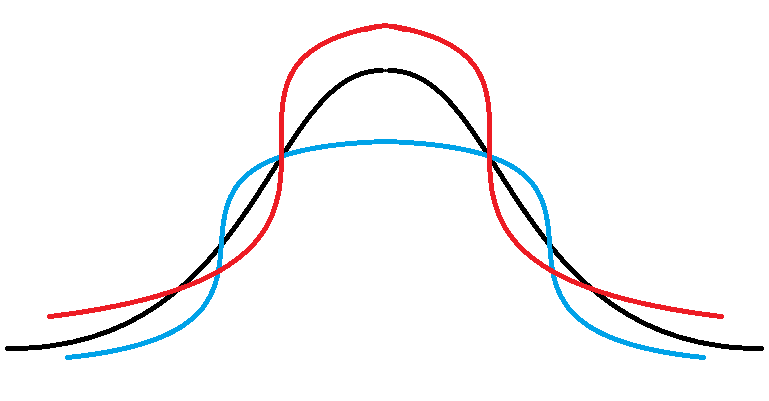
\includegraphics[height = 5cm]{chapter_6/files/Gaussians.png}

Our Kurtosis Method now leaves us with an optimization problem. Consider for a single source signal $S_i = W_i^TX$. We look for
\begin{align*}
    \max _{W_i} \quad & \text{Kurtosis}(W_i^TX) \\
    \text{s.t.} \quad & \text{Var}[W_i^T X] = 1 \\
            \quad & \mathbb{E}[W_i^TX] = 0
\end{align*}
\textbf{Remark: } \newline
- It turns out that most of the distribution we encounter are heavy-tails! So we choose to define a max problem.
\newline - It is sensitive to noise! Observe we have a $x^4$ term which enlarges any uncertainty in measurement.
\newline - The above max problem will find only one signal. To satisfy our purpose to find $k$ sources, we simply repeat it $k$ times, and each time we rule out previous results. Thus we find $k$ signals that are least Gaussian.


\subsection{Negative Entropy Method}
\textbf{Definition:} \textit{Entropy} is measure of uncertainty of a distribution and mathematically defined as $$H(p):=-\mathbb{E}_p[\log p]=-\int_x p(x)\log [p(x)]dx$$ \textbf{Remark: } \newline - This is Shannon's version of entropy definition (which is in fact axiomatically the correct version). 
\newline - It is a fact in Information Theory that among all distributions with a fixed variance, Gaussian has the highest entropy, which means least information is given.

\textbf{Setup: }\newline
Adopting the above idea of finding a least-Gaussian distribution, we maximize the negative entropy so that the distribution of $S_i$ gives most information, hence not looking like a Gaussian. We form an optimization problem as
\begin{align*}
    \max_W \quad & -H(W^TX) \\
    \text{s.t.} \quad & \text{Var}(W^TX)=1 \\
                \quad & \mathbb{E}(W^TX) = 0
\end{align*}


\subsection{Mutual Information Method}
\textbf{Definition: } Consider two random variables $X$ and $Y$. The \textit{mutual information} of $X$ and $Y$ is \begin{align*}
    I(x,y) = \int _x \int _y p(x,y) \log \frac{p(x,y)}{p(x)p(y)} \text{d}x \text{d}y
\end{align*}

Note that if $X$ and $Y$ are independent, we would have $I(X,Y) = 0$.

\textbf{Setup:}
Same idea as above, We minimize the mutual information between some distribution $X$ and a Gaussian. Hence, the corresponding optimization problem is
\begin{align*}
    \min \sum _{i<j} (W_i^TX,W^T_jX)
\end{align*}

\subsection{Summary}
The above are three methods commonly used in matrix factorization problems. In general, assume a data matrix $X$ has factorization $X = UV$. We treat $U$ as some transformation of source matrix $V$. Readers in fact have seen familiar problems before. 

- For example, in PCA, $X$ is the high-dimensional data, $U$ is the mapping for low dimensional data $V$. We want to minimize $\left\lVert X - UV\right\rVert^2_F$.

- Consider if Netflix is trying to figure out relation between shows and ratings. Let $X$ be the rating data which is generated by user and genre. Each user rates the movies which he has seen.
Let $R_{ij}$ be the rating assigned by user $i$ to movies $j$. Note if we assume that each user can only rate few movies, the $U$ matrix is super-sparse. We assume there are $k$ factors which have vital influence on users and movies, these factors maybe genre or something else. Define $U$ being the matrix of users and $M$ being the matrix of movies, we have objective function 
\begin{align*}
&\min_{U,M}\sum_{r_{ij} \text{ observed}}(r_{if} - u_im_j)\\
\text{Or equivalently: } & \min_{U,M} \left\lVert R - UM\right\rVert^2_F
\end{align*}

- Dictionary learning is another problem falls in this field. We want to summarize data to some small ``dictionary" to represent large data set with ``richness" preserved.

However, if we treat $U$ as linear transformation more than a matrix, we may ask think that $U$ does not have to be linear. This motivates out further study of non-linear dimensionality reduction methods.
